% --------------------------------------------------
% MG-Template for thesis, FEB 2020 v.1
% Das Dokument muss mit XeLaTeX kompiliert werden.
% --------------------------------------------------

% TODO: Paragraphüberschrift fett drucken
% TODO: Sprache auf Deutsch stellen
% TODO: ß soll nicht als SS sondern als ß angezeigt werden
% TODO: komplette Rechtschreibprüfung

\documentclass[openright, twoside, utf8, 11.5pt]{scrbook}

% \usepackage[german]{babel}
% \usepackage[utf-8]{inputenc}
\usepackage{amsmath}
\usepackage{lipsum}
\usepackage{mgthesis}
\usepackage{siunitx}

\sisetup{locale = DE}

\newcommand{\thesistype}{Projektarbeit}
\newcommand{\degreetype}{Bachelor/Master of Science (M./B.\,Sc.)}

\title{Qualitativer Vergleich von Beaterkennungsalgorithmen}
\author{Hannes Frank}
\date{19. Juli 2020}

\newcommand{\matnr}{4501110}
\newcommand{\gutachter}{Prof. Dr.-Ing. habil. Rainer Groh}
\newcommand{\betreuer}{M. Sc. Lars Engeln}


\begin{document}
	\color{mycolor}
	% Abkürzungen (für Verzeichnis: \acro statt \acrodef und mit begin/end{acronym} vor das Inhaltsverzeichnis bauen)
	\acrodef{RS}{Recommender Systems}
	\acrodef{CF}{Collaborative Filtering}
	\acrodef{DAW}{Digital Audio Workstation}
	\acrodef{IR}{Information Retrieval}
	\acrodef{ML}{Machine Learning}
	\acrodef{MCI}{Mensch-Computer-Interaktion}
	\acrodef{UX}{User Experience}
	\acrodef{UI}{User Interface}
	\acrodef{GUI}{grafische Benutzeroberfläche}
	\acrodefplural{GUI}[GUI]{grafischen Benutzeroberfläche}
	\acrodef{SUI}{Suchinterface}

	% Titelseite
	\makeatletter
\begin{titlepage}
	\RaggedRight
	\includegraphics[width=0.35\textwidth]{resources/logoTUD.png}\par\vspace{0cm}
	\noindent\rule{\textwidth}{0.4pt}
	{\normalfont\mdseries\small\sffamily Fakultät Informatik,}
	{\normalfont\mdseries\small\sffamily Institut für Software- und Multimediatechnik, Professur für Mediengestaltung}
	\vspace{2mm}\noindent\hrule
	\vspace{3cm}
	{\normalfont\Large \thesistype \par}
	\vspace{1cm}
	{\normalfont\Huge\mdseries\sffamily \@title\par}
	\vspace{1.5cm}
	{\normalfont\large im Rahmen des Moduls:\par}
	{\normalfont\Large\bfseries INF-D-960 Analyse eines Forschungsthemas \par}
	\vspace{1cm}
	{\sffamily\large\mdseries erarbeitet von\par}
	\vspace{1.5mm}
	{\normalfont\Large \@author\par}
	\vspace{0.5mm}
	{\normalfont\large Matrikelnummer: \matnr \par}
	\vspace{3.0cm}
	{\sffamily\large Gutachter:\par}
    \vspace{1mm}
	{\normalfont\large \gutachter \par}
	\vspace{7mm}
	{\sffamily\large Betreuer:\par}
	\vspace{0.7mm}
	{\normalfont\large \betreuer \par}
	\vspace{1cm}
	{\sffamily\large\mdseries eingereicht am\par}
	\vspace{1mm}
	{\normalfont\normalsize \@date \par}
\end{titlepage}
\makeatother


	\cleardoublepage
	\begingroup
		\renewcommand*{\chapterpagestyle}{empty}
		\pagestyle{empty}
		\makeatletter
\chapter*{Selbstständigkeitserklärung}

\justifying Hiermit erkläre ich, dass ich die vorliegende Arbeit mit dem Titel \\

\vspace{0.5cm}
\centering
{\large\sffamily\mdseries \@title } \\
\vspace{1.0cm}
\justifying

selbstständig und ohne die Benutzung anderer als der angegebenen Hilfsmittel angefertigt habe. Alle Stellen, die wortwörtlich oder sinngemä\ss\ aus veröffentlichten oder nicht veröffentlichten Quellen entnommen sind, sind als solche kenntlich gemacht.\\

\vspace{2.5cm}
%\hfill \rule{0.33\textwidth}{0.4pt}\par
Dresden, \@date \hfill \@author
\makeatother
			\newpage
			\pagestyle{empty}
			\null\newpage
		\chapter*{Kurzfassung}

Beaterkennungsalgorithmen sind Algorithmen,
	die den regelmä{\ss}igen Puls von Musikstücken erkennen,
	zu dem wir Menschen oft beim Hören von Musik unterbewusst mit dem Fu{\ss} oder einem Finger mittippen.
Viele dieser Algorithmen geben auch Schätzungen des Tempos des Musikstücks aus.
In dieser Arbeit wurden die drei Algorithmen
	von~\cite{2001_BeatThis}, \cite{2009_DaPlSt} und \cite{2011_PlRoSt}
	im Echtzeitbetrieb getestet und verglichen.
Dabei wurden sie auf
	Genauigkeit der Tempovorhersagen, Genauigkeit der Beatzeitpunkte, längste korrekte Beatfolge und benötigte Rechenzeit
	untersucht.
Es wurden Tests implementiert,
	die die Algorithmen auf mit Beatzeitpunkten annotieren Liedern eines Datensatzes laufen lassen
	und dabei deren Ausgaben aufzeichnen.
Die Auswertung dieser Aufzeichnungen ergab,
	dass \cite{2009_DaPlSt} in allen vier Tests am besten abgeschnitten hat.

		\newpage
			\pagestyle{empty}
			\null\newpage
		\tableofcontents
		\cleardoublepage
	\endgroup

	% Inhalt
	% include = newpage; input = samepage
	\mainmatter
	\chapter{Einleitung}
\label{einleitung}
\acresetall

In diesem Kapitel wird die Zielsetzung dieser Arbeit
	und das Beaterkennungsproblem kurz erlkärt
	sowie dessen Anwendungsgebiete vorgestellt.

\section{Kontext}
{
	% leicht für Menschen, schwer für Maschinen
	Die Erkennung der regelmä{\ss}igen Schläge des Taktes eines Musikstücks ist eine triviale Aufgabe für Menschen.
	Manchmal tippen wir sogar unterbewusst unseren Fu{\ss} zum Takt der Musik,
		ohne aktiv darüber nachzudenken.
	Es ist jedoch sehr schwer diese Aufgabe zu automatisieren,
		da Maschinen kein Taktgefühl haben.
	Dennoch gibt es verschiedene Algorithmen,
		die genau das bewerkstelligen.
	% Anwendungen
	Diese Beaterkennungsalgorithmen werden z. B. in Videobearbeitungssoftware verwendet,
		um die visuelle Spur automatisch mit der Audiospur zu synchronisieren.
	Deshalb werden besonders beim Erstellen von Musikvideos solche Algorithmen eingesetzt.
	Auch in Audiobearbeitungs- und Aufnahmesoftware finden Beaterkennungsalgorithmen Einsatz,
		z. B. bei der automatischen Indizierung von Musikstücken.
	Bei Liveauftritten spielen Beaterkennungsalgorithmen auch eine wichtige Rolle.
	Hier werden sie eingesetzt um z. B. die Bühnenbeleuchtung automatisch und passend zur Musik zu steuern.
}

\section{Zielsetzung}
{
	Ziel dieser Arbeit ist es,
		einen umfangreichen, qualitativen Vergleich von ausgewählten Beaterkennungsalgorithmen zu erstellen,
		der hilfreich für die Auswahl eines geeigneten Algorithmus für einen Anwendungsfall ist.
	Dazu wurden drei Algorithmen analysiert und implementiert
		und mehrere Vergleichstests erstellt.
	Die Tests lassen die Algorithmen auf mit Beatpositionen annotierten Musikstücken laufen,
		beobachten dabei deren Ausgabe
		und vergleichen sie mit den Annotationen der Lieder.
	Auf diese Art und Weise werden mehrere Metriken zur Bewertung der Algorithmen erstellt,
		anhand welcher die Algorithmen verglichen werden.
}

\section{Kapitelübersicht}
{
	In Kapitel~\ref{grundlagen} werden für diese Arbeit relevante musikalische Grundbegriffe vorgestellt
		und die Grundlagen der Beaterkennung beschrieben.
	In Kapitel~\ref{verwandte_arbeiten} werden alle Paper,
		die im Rahmen dieses Forschungsprojekts verwendet wurden,
		kurz vorgestellt.
	In Kapitel~\ref{analyse} wird die Auswahl der für den Vergleich verwendeten Algorithmen begründet
		und deren genaue Funktionsweise beschrieben.
	In Kapitel~\ref{konzept} werden die Ziele des Vergleichs definiert,
		sowie dessen Aufbau und Umsetzung aufgezeigt.
	In Kapitel~\ref{ergebnisse} werden die Ergebnisse aller Tests vorgestellt und interpretiert.
	Es werden zu jedem Test mögliche Erklärungen für dessen Ergebnis abgegeben.
	Dabei wird in jedem Abschnitt eine der vier Forschungsfragen aus Kapitel~\ref{konzept} adressiert.
	In Kapitel~\ref{zusammenfassung} werden das Ziel der Arbeit, die Umsetzung des Vergleichs und das Resultat der Tests kurz zusammengefasst.
	Abschlie{\ss}end werden Ziele für zukünftige Vergleiche von Beaterkennungsalgorithmen vorgestellt.
}


	\chapter{Grundlagen und Begriffe}
\label{grundlagen}

\section{Musikalische Grundbegriffe}
{
	Um die in dieser Arbeit untersuchten Beaterkennungsalgorithmen zu verstehen,
		wird etwas musikalisches Grundwissen benötigt.
	In diesem Abschnitt werden deshalbt Grundbegriffe erklärt,
		die in der restlichen Arbeit verwendet werden.

	\paragraph{Takt}
	{
		Fast jedes Musikstück ist zeitlich in kurze und gleichlange Abschnitte unterteilt.
		Diese Abschnitte nennt man Takte
			und sie geben der Musik eine gewisse Struktur,
			da sich oft bestimmte Muster, wie z.B. Schlagzeugrhythmen, in jedem oder jedem zweiten Takt wiederholen
			und auch die Grenzen von Strophe, Refrain usw. an Taktgrenzen orientiert sind.
		Die Länge eines Taktes hängt von der Taktart und dem Tempo des Stücks ab
			und ist meist im einstelligen Sekundenbereich.
	}

	\paragraph{Schlag (Beat)}
	{
		Ein Schlag (engl. Beat) ist eine Unterteilung des Taktes.
		Jeder Takt hat genau gleichviele Schläge (außer es gibt einen Taktartwechsel im Stück).
		Die Abfolge von Schlägen in einem Lied ist oft dieselbe,
			die ein Mensch beim Hören der Musik intuitiv mit dem Fuß mitklopfen würde.
	}

	\paragraph{Taktart}
	{
		Die Taktart besteht aus zwei Teilen
			und wird deshalb oft als ungekürzter Bruch angegeben (z. B. 4/4).
		Der Zähler gibt an aus wievielen Schlägen ein Takt besteht.
		Der Nenner gibt an wie lange ein Schlag dauert,
			jedoch nicht in einer Zeiteinheit sondern als Notenwert.
		Ein Nenner von 4 bedeutet z. B., dass ein Schlag so lange wie eine Viertelnote dauert.
		Das ist für die musikalische Notation relevant,
			hat aber keine Bedeutung für diese Arbeit,
			da dahinter kein Bezug zur tatsächen Dauer (in Sekunden) eines Schlages steckt.
		Die meisten Lieder haben einen 4/4-Takt,
			weshalb manche Algorithmen in dieser Arbeit speziell auf diese Taktart ausgelegt sind.
			% TODO: sagen welche Algorithmen genau
	}

	\paragraph{Tempo}
	{
		Das Tempo eines Musikstückes gibt an wie schnell es gespielt wird
			und bestimmt somit die tatsächliche Dauer (in Sekunden) eines Schlages.
		Es wird in BPM (engl. beats per minute) angegeben.
		Üblicherweise befinden sich Tempi von Musikstücken in einem Bereich zwischen 60 und 180 BPM.
	}
}

\section{Beaterkennung}
{
	Beaterkennung ist die Aufgabe aus rohen Audiodaten die Anfangszeitpunkte der einzelnen Schläge eines Musikstücks zu extrahieren.
	Zusätzlich wird von manchen Algorithmen auch das Tempo berechnet.

	\paragraph{}
	{
		Das Beaterkennungsproblem bringt folgende Herausforderungen mit sich:
	}

	\paragraph{1} % kein eindeutiges Beatgeräusch
	{
		Es gibt nicht immer ein bestimmtes Geräusch,
			dass die Anfangszeitpunkte der Schläge marktiert.
		Es kann sogar sein, dass auf einen Beat gar kein Signal kommt.
	}

	\paragraph{2} % Onsetungenauigkeit
	{
		Da oft viele Instrumente, mit sehr unterschiedlichen Klängen, in einem Lied speielen,
			ist es schwierig besonders genaue Einsatzzeitpunkte von Noten zu bestimmen.
	}

	\paragraph{3} % Echtzeit
	{
		Um die Beaterkennung in Echtzeit zu berechnen,
			können aus dem Eingangssignal nur Samples aus der Vergangenheit genutzt werden,
			statt das komplette Signal bei nicht-Echtzeit-Algorithmen.
	}

	\paragraph{4} % nicht trivial
	{
		Es ist nicht nützlich einfach die Lautstärkemaxima eines Audiosignals zur Beaterkennung zu nutzen,
			da es auch viele Peaks gibt,
			die nicht auf einen Beat passen.
	}

	\paragraph{5}  % Nichteindeutigkeit
	{
		Die Zuordnung von Audiodaten zu Beatzeitpunkten und Tempo ist nicht eindeutig.
		Schläge und Takte sind lediglich eine gedankliche Einteilung des Stücks,
			die man nicht direkt hören kann
			sondern sich nur dadurch bemerkbar macht,
			dass musikalische Ereignisse
			(z. B. Anfang und Ende einer Note, Schlagzeugtöne oder Harmoniewechsel)
			an deren Grenzen orientiert sind.
		Man könnte also z. B. ein Stück mit 160 BPM auch als eines mit 80 BPM betrachten
			(angenommen der Zähler der Taktart ist durch zwei teilbar),
			indem man jeweils zwei Takte als einen interpretiert.
		Das Audiosignal wäre bei beiden Varianten das gleiche.
	}


	% difficulties
	% * viele instrumente --> schwierig genaue Onsets zu bestimmen
	% * man kann nicht einfach den Peak picken um beats zu finden, weil da es auch viele Energy-Peaks an Stellen wo kein Beat is gibt
	% * ...
	% * ...
}

	\chapter{Verwandte Arbeiten}
\label{verwandte_arbeiten}
\acresetall

In diesem Kapitel werden alle Paper,
	die im Rahmen dieses Forschungsprojekts verwendet wurden,
	kurz vorgestellt.

% 1997 Goto, Muraoka - Issues in Evaluating Beat Tracking Systems
\paragraph{\cite{1997_GoMu1}}
{
	befasst sich mit Problemen bei der Bewertung von Beaterkennungsalgorithmen.
	Es wird eine Methode zur Evaluierung der Genauigkeit dieser Algorithmen vorgestellt,
		welche auch typische Fehler,
		die solche Systeme machen,
		in Betracht zieht.
	Diese Methode wird auch in dieser Arbeit verwendet.
}

% __________ ALGORITHMEN ______________________________________________________

% 2000 Dixon
\paragraph{\cite{2000_Di}}
{
	stellt einen vielversprechenden Algorithmus zur Erkennung von Beats vor,
		der auf der Häufigkeitsverteilung von Zeitintervallen zwischen den Beats basiert.
}

% 2001 Beat This
\paragraph{\cite{2001_BeatThis}}
{
	stellen einen Algorithmus vor,
		der das Tempo eines Musikstücks erkennt.
	Dieser wurde nicht für Echtzeitanwendungen konzipiert
		aber kann trotzdem dafür verwendet werden.
	Er basiert auf einer Kammfiltermatrix
		und hat generell einen relativ einfachen Aufbau im Vergleich zu den anderen Algorithmen in dieser Arbeit.
}

% 2001 Goto
\paragraph{\cite{2001_Go}}
{
	beschreibt ein komplexes Beaterkennungssystem,
		welches nicht nur Beatpositionen erkennt,
		sondern auch die hierarchische Taktstruktur eines 4/4-Taktes,
		welche aus Takten, halben Takten und viertlen Takten (Schlägen) besteht.
	Das System ist eine Kombination und Verbesserung zweier älterer Systeme,
		die zum einen für Musik mit Schlagzeug (\cite{1994_GoMu}, \cite{1995_GoMu1}, \cite{1998_GoMu})
		und zum anderen für Musik ohne Schlagzeug (\cite{1996_GoMu}, \cite{1997_GoMu2}, \cite{1999_GoMu})
		ausgelegt waren.
	Das neue System funktioniert sowohl mit Musik mit Schlagzeug als auch mit Musik ohne Schlagzeug.
	Au{\ss}erdem ist es vielversprechend,
		weil mehrere verschiedene Informationen verwendet werden,
		um die Ausgabe zu verbessern,
		namentlich die Einsatzzeitpunkte, Harmoniewechsel und gängige Schlagzeugmuster.
}

\paragraph{\cite{2004_BeDaDuSa}}
{
	vergleicht verschiedene \acp{ODF},
		welche wesentlicher Bestandteil vieler Beaterkennungsalgorithmen sind.
	Au{\ss}erdem wird eine \ac{ODF} vorgestellt,
		die sowohl auf Lautstärkeänderungen
		als auch auf Phasenänderungen in der komplexen Domäne
		reagiert.
	Diese \ac{ODF} wird auch in zwei der in dieser Arbeit verglichenen Algorithmen verwendet.
}

\paragraph{\cite{2009_DaPlSt}}
{
	präsentiert ein Beaterkennungssystem,
		das ein Hybrid aus zwei Vorgängern ist.
	So wurde die Beatzeitpunktbestimmung von~\cite{2007_El}
		und die Tempoerkennung von~\cite{2007_DaPl} inspiriert.
}

% 2011 PlRoSt
\paragraph{\cite{2011_PlRoSt}}
{
	erklärt einen echtzeitfähigen Beaterkennungsalgorithmus mit visuellem Interface.
	Hierbei wird eine intuitive Repräsentation einer Kammfiltermatrix visualisiert,
		mit der der Benutzer interagieren kann.
	Der Algorithmus kann auch ohne Nutzerinteraktion laufen,
		aber könnte dann Schwierigkeiten haben,
		die Mehrdeutigkeit des Beaterkennungsproblems aufzulösen.
}

% __________ DATENSATZ ________________________________________________________

\paragraph{\cite{2012_HoDaZaOlGo}}
{
	stellt eine Methode vor zur Identifikation von komplexer Musik,
		die für Beaterkennungsalgorithmen schwierig ist.
	Diese Methode wird benutzt,
		um einen schwierigen Datensatz für die Evaluation von Beaterkennungsalgorithmen zu erstellen.
	Es wird auch beschrieben,
		wie die einzelnen Lieder des Datensatzes annotiert wurden.
	Der so entstandene Datensatz wird auch in den Vergleichstests dieser Arbeit genutzt.
}

	\chapter{Analyse der Algorithmen}
\label{analyse}

\section{Selektion}
{
}

\section{Vergleich}
{
}

\section{Funktionsweise}
{
	% TODO: sagen, dass ich hier meine eigenen Implementierung beschreibe, welche aber dem Paper entsprechen sollte und wenn nicht schreib ichs dazu
	% TODO: vielleicht ein Wort zur Notation verlieren wegen Subscript und Klammern
	% * Subsxript t ist meistens Zeitreihenindex
	% * Subscripte sind meistens Indices für Zeitreihen, Arrays oder Matrizen
	% * manchmal werden Subscripte auch benutzt um verschiedene Versionen einer Variable zu differenzieren
	%   z. B. tau_f und tau_neu --> dann wern sa aber als Wörter geschrieben mit ner Text-Schriftart
	% * Zahlen in Klammern sind Parameter einer Funktion, die iwas mit diesen Zahlen macht
	% TODO: irgendwo erklären was ne ODF ist

	\subsection{2011 Plumbley, Robertson, Stark - Real-Time Visual Beat Tracking Using a Comb Filter Matrix}
	{
		\subsubsection*{Ein- und Ausgabe}
		{
			Der Algorithmus von \cite{2011_PlRoSt} bekommt als Eingabe ein rohes, PCM-kodiertes Audiosignal mit einer Abtastfrequenz von \SI{44.1}{\kilo\hertz}.
			Die Samples sind als 32-Bit Gleitkommazahlen kodiert.
			Die Ausgabe besteht aus Tempo $\gamma$ und Phase $\theta$ der erkannten Beatfolge
				und wird alle \num{11.61} Millisekunden aktualisiert.
			Aus dem Tempo ergibt sich die Beatperiode $T = 1 / \gamma$.
			Um die genaue Bedeutung der Phase zu verstehen,
				kann man die komplette Laufzeit des Algorithmus in $T$ lange Abschnitte unterteilen.
			So sollte sich in jedem Abschnitt ein Schlag befinden.
			Die Phase $\theta$ gibt an,
				wann innerhalb dieser Abschnitte der Schlag kommt (\SIrange{0}{360}{\degree}).
			Das ist zum Einen Hilfreich,
				um den genauen Zeitpunkt des nächsten Schlags zu bestimmen.
			Zum Anderen kann man an langsamen Drifts der Phase erkennen,
				ob das geschätzte Tempo ein bischen zu langsam oder zu schnell ist.
		}

		\subsubsection*{Funktionsweise}
		{
			% STFT und ODF
			Der Algorithmus  arbeitet ebenfalls mit einer Einsatzdetektionsfunktion (Abk.: ODF von engl. onset detection function).
			Tatsächlich verwent er sogar dieselbe komplexe Spektraldifferenzfunktion $d$ aus~\cite{2004_BeDaDuSa},
				die auch in \cite{2009_DaPlSt} verwendet wurde.
			Diese ODF bekommt einen STFT-Frame $p_t$ als Eingabe und gibt ein ODF-Sample $d_t$ zurück.
			\begin{equation}
				d_t = d(p_t)
			\end{equation}
			Für die Kurzzeit-Fouriertransformation wurde ein Von-Hann-Fenster mit einer Breite von \num{1024} und eine Schrittweite von \num{512} verwendet.
			Bei einer Abtastfrequenz von \SI{44.1}{\kilo\hertz} entsteht so ein neuer STFT-Frame,
				und somit auch ein neues ODF-Sample,
				alle $512 / \SI{44.1}{\kilo\hertz} = \SI{11.61}{\milli\second}$.

			% vorverarbeitete ODF
			Im nächsten Schritt werden die ODF-Samples vorverarbeitet.
			Dazu wird zuerst der Median der Einsatzdetektionsfunktion berechnet.
			Da aus~\cite{2011_PlRoSt} nicht hervorgeht, über welchen Zeitraum der Median berechnet wird,
				wird in meiner Implementierung,
				wie in~\cite{2009_DaPlSt},
				ein \num{6} Sekunden langer Analyserahmen der Einsatzdetektionsfunktion gespeichert
				und dieser zur Berechung des Medians genutzt.
			Anders als bei~\cite{2009_DaPlSt} wird hier der Analyserahmen nicht alle \num{1.5} Sekunden,
				sondern nach jedem neuen ODF-Sample weitergeschoben,
				sodass er immer die letzten \num{6} Sekunden (\num{517} Samples) der Einsatzdetektionsfunktion enthält.
			So wird aus jedem neuen ODF-Sample $d_t$ sofort das nächste Sample $v_t$ der vorverarbeiteten ODF berechnet.
			\begin{equation}
				v_t = v(d_t) =
				\begin{cases}
					d_t & \text{falls } d_t > \text{median} \\
					0    & \text{sonst}
				\end{cases}
			\end{equation}
			Diese vorverarbeitete Einsatzdetektionsfunktion wird im nächsten Schritt genutzt,
				um die Kammfiltermatrix zu aktualisieren.

			% Beschreibung Kammfiltermatrix
			Die Kammfiltermatrix $X_{\tau, x}$ enthält eine Zeile für jede mögliche Temposchätzung, die der Algorithmus abgeben kann.
			Diese werden mit der entsprechenden Beatperiode in ODF-Sample-Dauern adressiert.
			Da der Algorithmus auf einen Tempobereich von \SIrange{80}{160}{BPM} beschränkt ist,
				ergibt sich ein minimaler Zeilenindex von
				$\tau_{\text{min}} = \lfloor(\SI{11.61}{\milli\second} \cdot \SI{160}{\per\minute})^{-1}\rfloor = 32$
				und ein maximaler Zeilenindex von
				$\tau_{\text{max}} = \lceil(\SI{11.61}{\milli\second} \cdot \SI{80}{\per\minute})^{-1}\rceil = 65$.
			Jede Zeile entählt eine Zelle für jeden diskreten Zeitpunkt innerhalb der entsprechenden Beatperiode.
			Diese haben auch jeweils einen Abstand von einer ODF-Sample-Dauer
				und werden deshalb ebenfalls in dieser Einheit adressiert.
			So ergibt sich für eine bestimmte Zeile $\tau$ ein Zellenindexbereich von $x = 0, ..., \tau - 1$.
			Der Zellenindex $x$ ist direkt mit der Phase $\theta$ korreliert,
				jedoch wird hier eine andere Variable verwendet,
				da $x$ in ODF-Sample-Dauern von $0$ bis $\tau - 1$ ist
				und $\theta$ einen Phasenwinkel in von \SIrange{0}{359}{\degree} ist
				und die Umrechnung der beiden Größen von der Beatperiode $\tau$ abhängt.

			% Kammfiltermatrixaktuelisierung
			Die Kammfiltermatrix wird mit jedem neuen vorverarbeiteten ODF-Sample $v_t$ zum Zeitpunkt $t$ aktualisiert.
			Dabei wird für jede Zeile $\tau$ die Zelle,
				die den aktuellen Zeitpunkt entspricht $x = t \bmod \tau$,
				mit der Updateregel
				\begin{equation}
					X_{\tau, x} \leftarrow
						\alpha v_t +
						(1 - \alpha) \max_{\substack{\tau_m = \tau_{\text{min}}, ..., \tau_{\text{max}} \\ x_m = 0, ..., \tau - 1}}
							(g(\tau, \tau_m, 3.5) g(x, x_m, 6) X_{\tau, x})
				\end{equation}
				aktualisiert.
			Die Konstante $\alpha$ ist \num{0.1}
				und $g$ ist eine Gewichtsfunktion,
				die die Form einer gaußschen Normalverteilung annimmt,
				jedoch immer ein Maximum von \num{1} hat.
			$\sigma$ bestimmt also nur die Breite der Glockenkurve,
				aber nicht die Höhe,
				wie bei einer gewöhnlichen Normalverteilung.
			\begin{equation}
				g(c, m, \sigma) = e^{-\frac{(c - m)^2}{2\sigma^2}}
			\end{equation}

			% Idee dahinter
			Die Idee hinter dieser Updateregel ist,
				dass sich,
				in der zum richtigen Tempo gehörenden Zeile,
				die Peaks der vorverarbeiteten ODF immer wieder an der gleichen Stelle überlagern
				und somit eine Zelle in dieser Zeile einen sehr hohen Wert annimmt,
				während in anderen Zeilen,
				wegen des unpassenden Tempos dieser Zeilen,
				die Peaks immer auf eine andere Stelle treffen
				und es so nicht schaffen eine einzelne Zelle hochzudrücken.
			Um das geschätzte Tempo und die Phase zu bestimmen,
				kann man nach dem Maximum in der Matrix suchen.
			Bevor das geschiet,
				durchläuft diese jedoch erst einen weiteren Verarbeitungsschritt.

			% Y-Matrix
			Zunächst wird jede Zeile mit einem Rayleigh-Gewicht multipliziert.
			Diese Gewichtsfunktion hat ihr Maximum bei \SI{120}{BPM} und flacht nach außen hin ab.
			So werden häufiger vorkommende Tempi, bevorzugt.
			Die Rayleigh-Funktion ist wie folgt definiert:
			\begin{equation}
				r(\tau) = \frac{\tau}{\beta^2}e^{\frac{-\tau^2}{2\beta^2}}
			\end{equation}
			wobei die Konstante $\beta$ den höchsten Punkt der Gewichtsfunktion bestimmt.
			Ein Wert von $\beta = 43$ ODF-Samples entspricht hier einem Tempo von
				$(43 \cdot \SI{11.61}{\milli\second})^{-1} = \SI{120}{\per\minute}$.
			Die Zeile des rightigen Tempos hat wahrscheinlich eine starke Konzentration an hohen Werten um den Punkt der richtigen Phase herum.
			Das bedeutet,
				dass diese Zeile eine niedrigere Entropie hat als andere Zeilen,
				deren Werte gleichmäßiger über die gesamte Zeile verteilt sind.
			Die Entropie einer Matrixzeile ist durch
				\begin{equation}
					h(\tau) = \sum_{x = 0}^{\tau - 1} -p(\tau, x) log(p(\tau, x))
				\end{equation}
				definiert, wobei
				\begin{equation}
					p(\tau, x) = \frac{X_{\tau, x}}{\sum_{x_i = 0}^{\tau - 1}X_{\tau, x_i}}
				\end{equation}
				als Häufigkeitsverteilung einer Zeile interpretiert werden kann.
			Als nächstes wird in der resultierenden Matrix
				\begin{equation}
					Y_{\tau, x} = \frac{r(\tau)}{h(\tau)}X_{\tau, x}
				\end{equation}
				nach dem Maximum gesucht.
			Der Matrixindex $(\tau_{\text{neu}}, x_{\text{neu}})$ des Maximums gibt das wahrscheinlichste Tempo und die wahrscheinlichste Phase an.

			% Tempoübergänge
			Da das so ermittelte Tempo-Phase-Paar  z. B. bei Unregelmäßigkeiten in der Musik etwas hin und her springen kann,
				gibt es noch eine Tempoupdateregel,
				die dafür sorgt,
				dass sich das Tempo und die Phase nur dann ändern können,
				wenn entweder die neue Hypothese sich in der Matrix relativ nah an der alten befindet,
				oder sie viel stärker ist als die alte.
			Hierfür definieren wir eine Gewichtsfunktion,
				welche Werte in der Nähe der aktuellen Hypothese $(\tau_\text{f}, x_\text{f})$ bevorzugt.
			\begin{equation}
				w(\tau_{\text{neu}}, x_{\text{neu}}) =
					g(\tau_\text{f}, \tau_{\text{neu}}, 4)
					g(x_\text{f}, x_{\text{neu}}, 10)
			\end{equation}
			Die Standartabweichungen von \num{4} und \num{10} wurden durch~\cite{2011_PlRoSt} experimentell ermittelt.
			Die aktuelle Hypothese wird mit folgender Updateregel aktuelisiert:
			\begin{equation}
				(\tau_\text{f}, x_\text{f}) \leftarrow
				\begin{cases}
					(\tau_{\text{neu}}, x_{\text{neu}}) &
						\text{falls } w(\tau_{\text{neu}}, x_{\text{neu}}) Y_{\tau_{\text{neu}}, x_{\text{neu}}} >
							Y_{\tau_\text{f}, x_\text{f}} \\
					(\tau_\text{f}, x_\text{f}) &
						\text{sonst}
				\end{cases}
			\end{equation}

			% Schlusssatz
			All diese Berechnungen werden für jedes neue Sample der Einsatzdetektionsfunktion durchgeführt.
			So gibt der Algorithmus alle \SI{11.61}{\milli\second} eine neue Tempo-Phase-Hypothese aus.
		}
	}
}

	\chapter{Konzept}
\label{konzept}
\acresetall

In diesem Kapitel werden die Ziele des Vergleichs definiert,
	sowie dessen Aufbau und Umsetzung aufgezeigt.

% Wie funktionieren die Tests, ganz grob?
Um die drei Algorithmen zu vergleichen,
	werden verschiedene Tests durchgeführt.
Diese speisen verschiedene Lieder eines Testdatensatzes in die jeweiligen Algorithmen ein
	und nehmen dabei deren Ausgabe auf.
Aus diesen Testaufzeichnungen werden Metriken berechnet,
	die es ermöglichen,
	die Algorithmen miteinander zu vergleichen.

% Abschnittübersicht
In Abschnitt~\ref{konzept/ziele} wird erklärt,
	was die Ziele der einzelnen Tests sind
	und welche Fragen durch die Tests beantwortet werden sollen.
In Abschnitt~\ref{konzept/testdaten} wird der verwendete Datensatz vorgestellt
	und in Abschnitt~\ref{konzept/gestaltung} wird die Umsetzung der Tests beschrieben.

\section{Ziele} \label{konzept/ziele}
{
	Bevor man sinnvolle Vergleichstests konzipieren kann,
		muss zuerst festgestellt werden,
		unter welchen Gesichtspunkten die Algorithmen verglichen werden können.

	% Tempo
	Alle drei Algorithmen geben eine Schätzung des Tempos des aktuellen Songs aus.
	Daraus ergibt sich follgende die erste Forschungsfrage.
	\begin{equation}
		\label{question:tempo}
		\text{\emph{Wie hoch ist die Genauigkeit der Temposchätzungen?}}
	\end{equation}

	% Beatzeitpunkte
	Au{\ss}erdem liefern die Algorithmen von~\cite{2009_DaPlSt} und~\cite{2011_PlRoSt} zusätzlich noch Informationen zur Position des aktuellen oder nächsten Beats.
	So gibt~\cite{2011_PlRoSt} beispielsweise die Phase aus,
		welche die Position des Beats innerhalb des aktuellen Beatintervalls angibt.
	Daraus lassen sich die absoluten Beatzeitpunkte berechnen.
	Da das System von~\cite{2009_DaPlSt} direkt absolute Beatzeitpunkte ausgibt,
		können diese als Grundlage für einen weiteren Vergleich der beiden Algorithmen verwendet werden.
	Dies wirft zwei weitere Forschungsfragen auf.
	\begin{align}
		\label{question:beat}
		\text{\emph{Wie hoch ist die Genauigkeit der Vorhersage der Beatzeitpunkte?}} \\
		\label{question:streak}
		\text{\emph{Wie lang ist die längste korrekt bestimmte Beatfolge?}}
	\end{align}

	% CPU-Zeit
	Alle Algorithmen nutzen Ressourcen der \ac{CPU}.
	Folglich kann untersucht werden,
		welcher Algorithmus am effizientesten damit umgeht.
	Vor diesem Hintergrund reiht sich eine letzte Forschungsfrage ein.
	\begin{equation}
		\label{question:cpu_time}
		\text{\emph{Wie viel \acs{CPU}-Zeit wird im Echtzeitbetrieb pro Sekunde benötigt?}}
	\end{equation}
}

\section{Testdaten} \label{konzept/testdaten}
{
	% allgemeines Gelaber
	Als Testdatensatz wurde der Datensatz von~\cite{2012_HoDaZaOlGo} verwendet,
		da es einer der wenigen Datensätze ist,
		der frei erhältlich ist
		und per Hand mit Beatzeitpunkten annotiert ist.
	Um die Leistungsfähigkeit von Beaterkennungsalgorithmen bestimmen zu können,
		ist es wichtig,
		einen manuell annotierten Datensatz zu verwenden.
	Wäre der Datensatz automatisch annotiert worden,
		würde man nur den eigenen Beaterkennungsalgorithmus mit dem,
		der für die Annotation verwendet wurde,
		vergleichen.

	% Woher kommen die Daten?
	Der verwendete Datensatz wurde aus Audio-\acsp{CD} (\aclp{CD}) extrahiert.
	\acused{CD}
	Folglich haben alle Dateien eine Abtastfrequenz von \SI{44.1}{\kilo\hertz}
		und es ist kein Resampling notwendig.
	Aus den \acp{CD} wurden von jedem Song \SI{40}{\second} extrahiert.
	% Art der Musik
	Die Auswahl der Lieder beschränkt sich ausschlie{\ss}lich auf westliche Musik.
	Dabei sind verschiedene Musikrichtungen vertreten,
		unter anderem: Klassik, Romantik, Filmmusik, Blues, Chanson und Sologitarrenkompositionen.
	% Wie groß?
	Der Datensatz besteht aus 217 Liedern.
	Davon haben 19 Lieder einen einfachen leicht erkennbaren Rhythmus.
	% Warum schwierige Rhythmen?
	Viele bisherige Datensätze enthalten Musik aus Rock-, Pop- oder Dance-Genres
		mit leicht erkennbaren Beats,
		die klar durch Schlagzeugtöne definiert sind.
	Dies erleichtert den Beaterkennungsalgorithmen,
		die korrekten Beatzeitpunkte zu finden.
	Da aktuelle Systeme auf den einfachen Datensätzen bereits fast perfekte Ergebnisse erzielen,
		bleibt somit kaum Spielraum für weitere Verbeserung.
	Um dem entgegenzuwirken,
		haben die Autoren dieses Datensatzes absichtlich schwierige Rhythmen ausgewählt.

	% Labels
	Zu jedem Exzerpt eines Liedes gibt es eine Annotationsdatei,
		welche die Liste der Beatzeitpunkte in diesem Lied enthält.
	Das Tempo des Liedes an einem bestimmten Zeitpunkt wird durch den Kehrwert des aktuellen Beatintervalls bestimmt.
}

\section{Gestaltung der Tests} \label{konzept/gestaltung}
{
	Die Testsoftware besteht aus zwei Komponenten:
		Datenakquisition und Datenauswertung.

	\subsection{Datenakquisition}
	{
		% Was die Datenakquisition grob macht
		Die Datenakquisitionskomponente ruft die einzelnen Beaterkennungsalgorithmen auf
			und wurde in C++ implementiert
			um sie mit den Algorithmen zu linken.
		Es wird jedes Lied im Testdatensatz einmal in jeden der drei Algorithmen gegeben
			und dabei deren Ausgaben in einer \acs{CSV}-Datei (\acl{CSV}) gespeichert.
		\acused{CSV}
		Dabei entsteht eine Datei pro Lied und Algorithmus.
		Die Algorithmen werden vor jedem Song neu initialisiert.

		% Was bei welchem Alg. aufgezeichnet wird und wie
		Bei~\cite{2001_BeatThis} wird nur jede neue Tempovorhersage aufgezeichnet.
		Bei~\cite{2009_DaPlSt} und~\cite{2011_PlRoSt} werden zusätzlich die vorhergesagten Beatzeitpunkte gespeichert.
		Die Tempovorhersagen von~\cite{2011_PlRoSt} werden nur dann gespeichert,
			wenn sie sich im Vergleich zur letzten Tempovorhersage geändert haben.
		Da der Algorithmus alle \SI{11.61}{\milli\second} eine neue Tempovorhersage ausgibt,
			ist das bei diesem Algorithmus notwendig,
			um die Grö{\ss}e der \acs{CSV}-Dateien zu reduzieren.
		Da \cite{2011_PlRoSt} nicht direkt Beatzeitpunkte ausgibt,
			sondern eine Beatperiode $T$ und Phase $x$,
			welche ständig aktualisiert werden,
			wird anhand dieser Information der nächste Beatzeitpunkt berechnet
			und erst dann gespeichert,
			wenn er erreicht wird.
		Somit wird sichergestellt,
			dass jede Beatvorhersage nur einmal in der \acs{CSV}-Datei auftritt.
		Gibt es ein $k \in \mathbb{N}$, das die Gleichung $kT + x = t$ erfüllt,
			wobei $t$ der aktuelle Zeitpunkt ist,
			dann wird $t$ als Beatzeitpunkt gespeichert.

		% CPU-Zeit-Messung
		Die \ac{API} der Beaterkennungsalgorithmen funktioniert so,
			dass jedes Audiosample separat und nacheinander per Funktionsaufruf in das System gegeben wird.
		Alle Berechnungen laufen in Subroutinen dieser Funktion ab.
		Um die Gesamtrechenzeit des Algorithmus zu bestimmen,
			wird die \acs{CPU}-Zeit von jedem dieser Funktionsaufrufe gemessen und aufsummiert.
	}

	\subsection{Datenauswertung}
	{
		% allgemeines Gelaber
		In der Datenauswertungskomponente der Testsoftware werden lediglich die gespeicherten \acs{CSV}-Dateien verarbeitet.
		So konnte diese unabhängig von der Implementierung der Algorithmen und deren Programmiersprache programmiert werden.
		Hier entstehen vier Auswertungen,
			welche sich auf die vier Forschungsfragen aus Abschnitt~\ref{konzept/ziele} beziehen.

		\subsubsection*{Tempofehler}
		{
			% Wie Tempofehler berechnet werden
			Um die Genauigkeit der Temposchätzungen zu bestimmen,
				wird ein Fehlerhistogramm der Temposchätzungen erstellt.
			Dazu muss zunächst für jeden Algorithmus eine Liste aller Fehlerwerte erstellt werden.
			Es wäre es nicht zielführend für jede Temposchätzung einen Fehlerwert zu berechnen,
				da die einzelnen Algorithmen ihre Temposchätzungen in unterschiedlichen Abständen aktualisieren.
			Gibt~\cite{2011_PlRoSt} beispielsweise ein konstant falsches Tempo über einen längeren Zeitraum aus,
				würde er nur einmal ein Fehlerwert in dessen Fehlerliste eingetragen werden,
				während einer der anderen beiden Algorithmen
				für jede einzelne falsche Temposchätzung in diesem Zeitraum
				einen Fehlerwert in dessen Liste eingetragen bekommen würde.
			Aus diesem Grund wird ein Fehlerwert für jedes Beatintervall berechnet.
			So enthalten am Ende alle drei Fehlerlisten gleich viele Fehlerwerte.
			Das korrekte Tempo wird aus dem Kehrwert des aktuellen Beatintervalls berechnet,
				welches wiederum aus der Differenz des nächsten und des letzten Beatzeitpunktes bestimmt wird.
			Der Fehlerwert des aktuellen Intervalls ergibt sich aus der Differenz der aktuellen Tempovorhersage und dem korrekten Tempo.
			Alle Temposchätzungen vor dem ersten und nach dem letzten Beat werden ignoriert,
				da für diese Bereiche kein korrektes Tempo bestimmt werden kann.
			Gibt es im aktuellen Beatintervall keine Temposchätzung,
				wird die vorherige Schätzung genommen
				bzw. dieses Intervall übersprungen,
				wenn es bis zum aktuellen Zeitpunkt noch keine Schätzung gab.
			Gibt es mehrere Temposchätzungen,
				wird der Mittelwert genommen.

			% Halb- und Doppeltempofehler
			Da das Problem der Tempobestimmung nicht eindeutig ist,
				treten bei solchen Systemen verhäuft Halb- und Doppeltempofehler auf.
			Damit ist gemeint,
				dass der Algorithmus genau die Hälfte bzw. das Doppelte des richtigen Tempos schätzt.
			Liegt das korrekte Tempo au{\ss}erhalb des Wertebereichs
				(\SI{80}{\ac{BPM}} bis \SI{160}{\ac{BPM}} bei allen Algorithmen in dieser Arbeit),
				ist die beste Ausgabe eines Algorithmus,
				zwangsläufig das halbe oder doppelte Tempo.
			Um solche Fehler zu berücksichtigen,
				wird für jedes Beatintervall nicht nur die Differenz zum korrekten Tempo,
				sondern auch die Differenz zum halben und zum doppelten Tempo berechnet.
			So entstehen pro Song und Algorithmus drei Fehlerlisten.
			Die Liste mit der kleinsten Summe der Quadrate der Fehlerwerte wird der Gesamtfehlerliste des Algorithmus angehangen.
			Die Gesamtfehlerliste kann anschlie{\ss}end als Histogramm dargestellt werden.
		}

		\subsubsection*{\large Beatzeitpunktfehler und längste korrekte Beatfolge}
		{
			% Pairing
			Für die Bestimmung der Beatzeitpunktfehler muss zunächst
				für jeden korrekten Schlag $C_n$ der dazugehörige Schlag in der Ausgabe des Algorithmus $B_n$ gefunden werden.
			Dafür wird der Ansatz des Pairings von~\cite{1997_GoMu1} verwendet.
			Es werden für jeden korrekten Beat $C_n$ alle ausgegebenen Beats $B_m$ gesucht,
				die die folgende Ungleichung erfüllen.
			\begin{equation}
				C_n - \frac{1}{2}(C_n - C_{n - 1}) \le B_m < C_n + \frac{1}{2}(C_{n + 1} - C_n)
			\end{equation}
			Gibt es kein $B_m$,
				welches die Ungleichung erfüllt,
				wird $C_n$ als ungepaart markiert.
			Falls es genau ein $B_m$ gibt,
				welches die Ungleichung erfüllt,
				wird ein Paar $(C_n, B_m)$ gebildet.
			Werden für ein $C_n$ mehrere mögliche $B_m$ gefunden,
				dann bildet $C_n$ ein Paar mit dem $B_m$,
				das den kleinsten Paarfehler erzielt.
			Die anderen $B_m$ werden als ungepaart markiert.

			% Paarfehler
			Für jedes Paar $(C_n, B_m)$ wird ein normalisierter Paarfehler $P$ berechnet,
				der zwischen \num{0} und \num{1} liegt,
				wobei \num{0} bedeutet,
				dass $B_m$ genau auf dem korrekten Beat $C_n$ liegt,
				und \num{1},
				dass $B_m$ genau in der Mitte zwischen dem korrekten und dem nächsten oder vorherigen Beat liegt.
			\begin{equation}
				P((B_m, C_n)) =
					\begin{cases}
						\frac{2|B_m - C_n|}{C_{n + 1} - C_n} & \text{falls } B_m \ge C_n \vspace{3mm} \\
						\frac{2|B_m - C_n|}{C_n - C_{n - 1}} & \text{falls } B_m  <  C_n
					\end{cases}
			\end{equation}
			Alle ungepaarten Beats,
				sowohl aus $C_n$ als auch aus $B_n$,
				erhalten einen Fehlerwert von \num{1}.

			\begin{figure}[h]
				\centering
				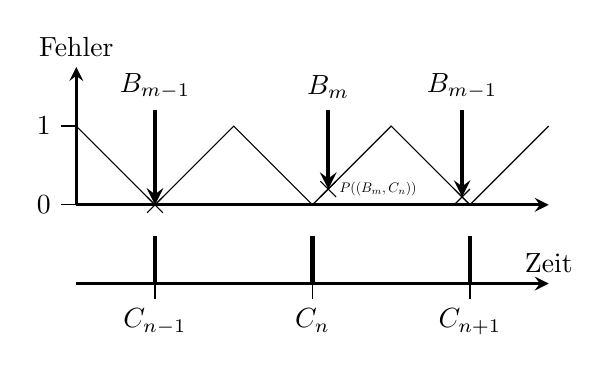
\begin{tikzpicture}
					\tikzstyle{axis} = [very thick, ->, >=stealth]
					\tikzstyle{tick} = [thin];
					\tikzstyle{cbeat} = [ultra thick]
					\tikzstyle{bbeat} = [ultra thick, ->, >=stealth]
					\tikzstyle{graph} = []

					\draw [axis] (0, -1) -- (6, -1) node [anchor=south] {Zeit};
					\draw [axis] (0, 0) -- (6, 0);
					\draw [axis] (0, 0) -- (0, 1.75) node [anchor=south] {Fehler};

					\draw [tick] (0, 0) -- (-0.2, 0) node [anchor=east] {0};
					\draw [tick] (0, 1) -- (-0.2, 1) node [anchor=east] {1};
					\draw [tick] (1, -1) -- (1, -1.2) node [anchor=north] {$C_{n - 1}$};
					\draw [tick] (3, -1) -- (3, -1.2) node [anchor=north] {$C_n$};
					\draw [tick] (5, -1) -- (5, -1.2) node [anchor=north] {$C_{n + 1}$};

					\draw [graph] (0, 1) -- (1, 0) -- (2, 1) -- (3, 0) -- (4, 1) -- (5, 0) -- (6, 1);

					\draw [cbeat] (1, -0.4) -- (1, -1);
					\draw [cbeat] (3, -0.4) -- (3, -1);
					\draw [cbeat] (5, -0.4) -- (5, -1);

					\draw [bbeat] (1, 1.2) node [anchor=south] {$B_{m - 1}$} -- (1, 0);
					\draw [tick] (0.9, -0.1) -- (1.1, 0.1);
					\draw [tick] (0.9, 0.1) -- (1.1, -0.1);
					\draw [bbeat] (3.2, 1.2) node [anchor=south] {$B_m$} -- (3.2, 0.2) node [anchor=west] {\scalebox{0.5}{$P((B_m, C_n))$}};
					\draw [tick] (3.1, 0.1) -- (3.3, 0.3);
					\draw [tick] (3.1, 0.3) -- (3.3, 0.1);
					\draw [bbeat] (4.9, 1.2) node [anchor=south] {$B_{m - 1}$}-- (4.9, 0.1);
					\draw [tick] (4.8, 0.0) -- (5.0, 0.2);
					\draw [tick] (4.8, 0.2) -- (5.0, 0.0);
				\end{tikzpicture}
				\caption{normalisierter Paarfehler $P$}
			\end{figure}

			% Halb-, Doppeltempo- und Pi-Phase-Fehler
			Beim Erkennen von Beatfolgen
				treten neben Halb- und Doppeltempofehler auch häufig $\pi$-Phase-Fehler auf.
			Davon ist die Rede,
				wenn der Beaterkennungsalgorithmus immer genau die Mitte zwischen zwei Beats als Beatvorhersage ausgibt.
			Dies tritt häufig bei Liedern auf,
				die zwischen den Hauptschlägen zusätzlich Off-Beat-Schläge haben,
				welche lauter bzw. prägnanter sind als die Hauptschläge.
			Um diese drei Fehlertypen und alle Kombinationen dieser Fehler zu berücksichtigen,
				werden pro Song sechs als korrekt angesehene Beatfolgen betrachtet:
				die originale Beatfolge,
				die Halbtempobeatfolge, in der jeder zweite Beat fehlt,
				die Doppeltempobeatfolge, in der zwischen jedem Beat ein weiterer Beat eingefügt wird
				und jeweils diese drei mit einer $\pi$-Phasenverschiebung.

			% Wie alles zusammen kommt
			Eine korrekt vorhergesagte Beatfolge ist eine Folge von Paaren,
				die keine ungepaarten Beats in ihrem Zeitraum hat und
				kein Paar mit einem Fehlerwert von \num{0.35} oder mehr hat.
			Für jeden Algorithmus wird für jedes Lied im Datensatz das oben beschriebene Pairing und die Fehlerberechnung
				sechsmal durchgeführt:
				einmal für jede der sechs Beatfolgen.
			Dadurch entstehen sechs Listen von Beatpaaren.
			Die Liste mit der längsten korrekt vorhergesagten Beatfolge
				wird als die Beatpaarfolge für diesen Song und diesen Algorithmus genommen.
			Die Paarfehler dieser Beatpaarfolge werden einer Gesamtfehlerliste hinzugefügt,
				welche pro Algorithmus existiert und später als Histogramm dargestellt wird.
			Die Fehler der ungepaarten Beats werden ebenfalls dieser Gesamtfehlerliste hinzugefügt.
		}

		\subsubsection*{\large Rechenzeit}
		{
			Die relative Rechenzeit eines Algorithmus ergibt sich aus der Division der für alle Lieder benötigten \acs{CPU}-Zeit durch die gesamte Dauer aller Lieder.
			Diese Zahl gibt an,
				wie viele Sekunden \acs{CPU}-Zeit ein Algorithmus benötigt,
				um eine Sekunde Audiodaten zu verarbeiten
				und erreicht bei Echtzeitalgorithmen maximal einen Wert von \num{1}.
			Der Rechenzeittest wurde auf einer Intel-\ac{CPU} der Baureihe Core i5-3320M mit einer Taktrate von \SI{2.6}{\giga\hertz} durchgeführt.
			Die Implementierungen sind nicht auf eine parallele Verarbeitung optimiert
				und nutzen deshalb maximal einen Thread.
		}
	}
}

	\chapter{Ergebnisse und Auswertung}
\label{ergebnisse}

% TODO: entweder Bezug auf die Fragen aus Kapitel 5 nehmen oder se ganz weg lassen

\section{Tempofehler}
{
	\subsection{Ergebnisse}
	{
		\begin{figure}[h]
			\hspace{-2.8cm}
			\includegraphics[scale=0.45]{resources/tempo_error_histogram.png}
			\caption{
				oben: Histogramme der Tempofehler, \\
				unten: Anzahl der Lieder, bei denen das halbe/korrekte/doppelte Tempo erkannt wurde
			}
			\label{fig:tempoerror}
		\end{figure}

		% Beschreibung Abbildung Tempofehler
		Die Histogramme in Abbildung~\ref{fig:tempoerror} zeigen die Verteilung der Tempofehler aller Lieder pro Algorithmus.
		Der abgebildete Bereich von \SIrange{-100}{100}{BPM} ist in \num{40} Balken unterteilt.
		So umfasst jeder Balken eine Spanne von \SI{5}{BPM}.
		Die Balkendiagramme zeigen pro Algorithmus,
			bei wievielen Liedern das halbe, das korrekte oder das doppelte Tempo als Referenztempo genommen wurde.

		% Auffälligkeiten der Abblidung
		Man kann deutlich erkennen,
			dass die Algorithmen von~\cite{2001_BeatThis} und~\cite{2011_PlRoSt} im Durchschnitt das Tempo etwas zu schnell schätzen.
		\cite{2009_DaPlSt} hingegen weicht im Durchschnitt nur minimal von einem Fehler von 0 ab und
			hat mehr Fehler, die sehr nah an 0 sind.
		Am meisten gestreut sind die Fehler bei \cite{2001_BeatThis}.
		Die Fehler von~\cite{2009_DaPlSt} haben zwar eine etwas größere Streuung (Standardabweichung) als die von~\cite{2011_PlRoSt},
			trotzdem kann man aber sagen,
			dass~\cite{2009_DaPlSt} in diesem Vergleich die besten Tempovorhersagen macht,
			da der Durchschnittsfehler viel näher an 0 ist.

		\begin{figure}[h]
			\centering
			\includegraphics[scale=0.45]{resources/dataset_tempo_histogram.png}
			\caption{Tempoverteilung des Datensatzes}
			\label{fig:dataset_tempo}
		\end{figure}

		Auffällig ist außerdem,
			dass bei jedem Algorithmus die meisten Lieder mit dem doppelten Tempo erkannt wurden.
		Das ist hauptsächlich dem limitierten Ausgabebereich der Algorithmen von \SIrange{80}{160}{BPM} zu verschulden.
		Abbildung~\ref{fig:dataset_tempo} zeigt die Verteilung der Tempi aller Beatintervalle im Datensatz.
		Der grüne Bereich enthält \SI{44.44}{\percent} aller Beatintervalle
			und markiert den Tempobereich,
			den die Algorithmen direkt ausgeben können (\SIrange{80}{160}{BPM}).
		Der gelbe Bereich markiert den Tempobereich,
			den die Algorithmen mit Berücksichtigung von Halb- und Doppeltempofehler ausgeben können,
			also von \SIrange{40}{80}{BPM} und von \SIrange{160}{320}{BPM},
			und enthält \SI{51.45}{\percent} aller Beatintervalle,
			wobei sich die meisten davon im untern Tempoberiech befinden.
		Das erklärt,
			warum so viele Lieder mit doppeltem Tempo erkannt wurden.
		Der rote Berech ist alles was außerhalb von \SIrange{40}{320}{BPM} ist
			und markiert den Tempobereich,
			den die Algorithmen unmöglich bestimmen können.
		Dieser Bereich enthält \SI{4.11}{\percent} aller Beatintervalle.
	}

	\subsection{Auswertung}
	{

		% Mögliche Erklärung 1 (ODF)
		Eine mögliche Erklärung,
			warum~\cite{2001_BeatThis} ungenauere Tempovorhersagen macht,
			ist,
			dass der Algorithmus eine einfachere Einsatzdetektionsfunktion (ODF von engl. onset detection function) verwendet.
		Die ODF basiert auf einer Glättung und einer anschliesenden Differentiation.
		So werden nur schnelle Anstiege der Lautstärke extrahiert,
			während bei der ODF der anderen beiden Algorithmen auch die Änderungen der Phase im Signal berücksichtigt werden
			und so auch Tonänderungen,
			bei denen die Lautstärke gleich bleibt,
			als Einsätze erkannt werden.

		% Mögliche Erklärung 2 (Tempo Induction)
		Außerdem verwendet~\cite{2001_BeatThis} zur Tempobestimmung Kammfilter mit drei Zähnen,
			welche einen ähnlichen Effekt wie eine Autokorrelationsfunktion (ACF von engl. auto correlation function) haben.
		Bei der ACF wird das Signal mit einer verzögerten Version von sich selbst elementweise multipliziert.
		Bei diesem Kammfilter wird das Signal mit zwei verzögerten Versionen von sich selbst elementweise addiert.
		Beide Operationen haben den Effekt,
			dass sich,
			bei der richtigen Verzögerung,
			die regelmäsigen Peaks des Signals überlagern
			und so die Ausgabe einen großen Wert annimmt.
		Weil ein Signal,
			was sich beispielsweise alle $T$ Sekunden wiederholt,
			sich gleichzeitig auch alle $2T, 3T,$ usw. Sekunden wiederholt,
			entstehen in der ACF sowie in der Kammfilterausgabe mehrere Peaks jeweils bei Vielfachen des ersten Peaks.
		\cite{2001_BeatThis} hört an dieser Stelle auf
			und bestimmt einfach den größten Peak als Beatperiode des Songs,
			während die anderen Peaks ignoriert werden.
		\cite{2009_DaPlSt} hingegen multipliziert anschließend die Ausgabe der ACF mit mehreren Kammfiltern
			um die Abstände von äquidistanten Peaks in der ACF zu ermitteln.

		% 2009 vs. 2011 (vorverarbeitete ODF)
		Die Tempobestimmung von~\cite{2011_PlRoSt} lässt sich schwierig mit der der anderen beiden Algorithmen vergleichen,
			da sie auf einem komplett anderen Prinzip aufbaut.
		Es lässt sich aber in der Visualisierung der Algorithmen erkennen,
			dass die vorverarbeitete ODF von~\cite{2009_DaPlSt} deutlichere und prägnantere Peaks hat,
			als die von~\cite{2011_PlRoSt}.
		Das könnte teilweise die unterschiedlichen Ergebnisse dieser beiden Algorithmen erklären.

		% 2009 vs. 2011 (Einlaufzeit)
		Eine weitere Erklärung für die schlechteren Ergbnisse von~\cite{2011_PlRoSt} könnte eine längere Einlaufzeit sein.
		Vielleicht ist die Tempovorhersage am Ende des Songs nicht ungenauer als die von~\cite{2009_DaPlSt}
			und der Algorithmus braucht nur länger um darauf zu kommen,
			weshalb am Anfang des Songs viele Tempovorhersagen falsch seien könnten
	}
}

\section{Beatzeitpunktfehler}
{
	\begin{figure}[h]
		\includegraphics[scale=0.5]{resources/beat_positions.png}
		\caption{
			oben: Histogramme der Beatzeitpunktfehler, \\
			mitte: Verteilung der längsten korrekten Beatfolgen, \\
			unten: Anzahl der Lieder, bei denen die Beatfolge mit halbem/korrektem/doppeltem Tempo erkannt wurde.
		}
		\label{fig:beaterror}
	\end{figure}

	In Abbildung~\ref{fig:beaterror} oben ist die Verteilung der Fehler aller Beatpaare zu sehen,
		inklusive der Fehler der ungepaarten Schläge,
		welche immer \num{1} sind.
	Die Graphen in der Mitte zeigen eine vertikel gespiegelte kumulative Verteilunsfunktion.
	So kann man für jede Beatfolgenlänge ablsesen,
		in wievielen Liedern (prozentual) eine korrekte Beatfolge mit mindestens dieser Länge erkannt wurde.
	Die Balkendiagramme zeigen pro Algorithmus,
		bei wievielen Liedern eine Beatfolge mit halbem, korrektem oder doppeltem Tempo als Referenzbeatfolge genommen wurde.
	Ob die Referenzbeatfolge um $\pi$ phasenverschoben wurde, oder nicht, ist nicht zu sehen.
}

\section{längste korrekte Beatfolge}
{
	Die längste korrekte Beatfolge von~\cite{2009_DaPlSt} ist \num{86}.
	\cite{2011_RoPlSt} hingegen hat Beatfolge von \num{39} Schlägen korrekt erfasst.
}

\section{Rechenzeit}
{
}

	\include{chapter/07_diskussion}
	\include{chapter/08_fazit}

	% Anhang
	\renewcommand{\appendixtocname}{Anhang}
	\renewcommand{\appendixname}{Anhang}
	\renewcommand{\appendixpagename}{Anhang}
	\renewcommand\thesection{\Alph{section}}
	\renewcommand{\setthesection}{\Alph{section}}
	\setcounter{chapter}{0}

	\cleardoublepage
	\addappheadtotoc
	\let\appendixpagenameorig\appendixpagename
	\renewcommand{\appendixpagename}{\normalfont\sffamily\Huge\mdseries\appendixpagenameorig}
	\appendixpage

	\begin{appendices}
		\begin{subappendices}
			\chaptermark{Literaturverzeichnis}
			\bibliography{references}
			\renewcommand{\listfigurename}{B \hspace{2.25mm} Abbildungsverzeichnis}
			\newpage
			\markboth{Abbildungsverzeichnis}{Abbildungsverzeichnis}
			\listoffigures
			\renewcommand{\listtablename}{C \hspace{2.25mm} Tabellenverzeichnis}
			\newpage
			\listoftables
			\markboth{Tabellenverzeichnis}{Tabellenverzeichnis}
		\end{subappendices}
	\end{appendices}
\end{document}
\backmatter
